\documentclass[wide,a4paper,titlepage,12pt] {article}
\usepackage{polski}
\usepackage[utf8]{inputenc}
\usepackage{listings}
\usepackage{slashbox}
\usepackage[table]{xcolor}
\usepackage{graphicx,pdflscape}
\usepackage{placeins}


\title{Urządzenia peryferyjne}
\author{Tymon Tobolski (181037)\\ Jacek Wieczorek (181043)}

% Title page layout (fold)
\makeatletter
\renewcommand{\maketitle}{
\begin{titlepage}
  \begin{center}
    \vspace*{3cm}
    \LARGE \@title \par
    \vspace{2cm}
    \textit{\small Autor:}\par
    \normalsize \@author\par \normalsize
    \vspace{3cm}
    \textit{\small Prowadzący:}\par
    Dr inż. Jacek Mazurkiewicz \par
    \vspace{2cm}
    Wydział Elektroniki\\ III rok\\ Pn 8.15 - 11.00\par
    \vspace{4cm}
    \small \@date
  \end{center}
\end{titlepage}
}
\makeatother



\begin{document}
\maketitle

\section{Cel laboratorium}
\paragraph{}
Celem laboratorium było zapoznanie się z zasadą działania odbiornika GPS, sposobem jego połączenia się z komputerem, a także z możliwościami i budową protokołu $NMEA$.

\section{Odbiornik GPS}
\paragraph{}
Urządzenie jakie mieliśmy do dyspozycji jest odbiornik GPS firmy Nokia, model LD-1W. Urządzenie komunikowało się z komputerem za pomocą technologii Bluetooth, emulując port szeregowy, w naszym przypadku port $COM120$.

\section{Protokół NMEA}
\paragraph{}
Protokół NMEA jest protokołem komunikacji morskiej wykorzystywanym powszechnie w morskich urządzeniach nawigacyjnych oraz urządzeniach GPS. Transmisja danych następuje w postaci zdań, zakodowanych za pomocą znaków ASCII. Pojedyncza sekwencja składa się z ciągu o długości do 82 znaków, a rozpoczynana jest znakiem \$. Kolejne pola sekwencji określają identyfikator zadania i przesyłane dane. Skwencja kończy się symbolami $<CR><LF>$ (carriage return, line feed).

\paragraph{}
Jedną z najważniejszych sekwencji protokołu NMEA są GGA , RMC i GSA. Podczas laboratorium korzystaliśmy z danych zawartych w sekwencji GGA w celu okreslenia aktualnego położenia odbiornika GPS .
\paragraph{}
Przykład sekwencji GGA : \\
$\$GPGGA,123519,4807.038,N,01131.000,E,1,08,0.9,545.4,M,46.9,M,,*47$ 
\paragraph{}
Gdzie :
\begin{itemize}
	\item GGA - Global Positioning System Fix Data
	\item 123519 - czas pomiaru według (12:35:19 UTC)
	\item 4807.038, N - szerokość geograficzna 48 st 07.038' N
	\item 01131.000,E - długość geograficzna 11 st 31.00' E
	\item 1 - fix quality (1 - GPS)
	\item 08 - ilość satelit
	\item 0.9 - poziome rozcieńczenie pozycji
	\item 545.4,M - wysokość nad poziomem morza w metrach
	\item 46.9,M - wysokość geoid nad elipsodą WGS84
	\item puste -  czas w sekundach od ostatniej aktualizacji DGPS
	\item puste - identyfiaktor stacji DGPS
	\item *47 - suma kontrolna
\end{itemize}

\section{Program}
\paragraph{}
Napisana przez nas aplikacja miała za zadanie połączyć się z urządzeniem, odczytywać sekwencje wysyłane przez odbiornik GPS, parsować je i w rezultacie wyświetlać dane i lokować punkt na mapie. Językiem implementacji programu jest $C\#$.
\subsection{Połączenie z portem szeregowym}
W celu komunikacji aplikacji z portem szeregowym skorzystaliśmy z klasy $SerialPort$ .

\lstset{ %
    language=java,                % choose the language of the code
    basicstyle=\scriptsize,       % the size of the fonts that are used for the code
    numbers=left,                   % where to put the line-numbers
    numberstyle=\scriptsize,      % the size of the fonts that are used for the line-numbers
    stepnumber=10,                   % the step between two line-numbers. If it's 1 each line 
                                    % will be numbered
    numbersep=9pt,                  % how far the line-numbers are from the code
    % backgroundcolor=\color{white},  % choose the background color. You must add \usepackage{color}
    showspaces=false,               % show spaces adding particular underscores
    showstringspaces=false,         % underline spaces within strings
    showtabs=false,                 % show tabs within strings adding particular underscores
    % frame=single,                 % adds a frame around the code
    % tabsize=2,                  % sets default tabsize to 2 spaces
    % captionpos=b,                   % sets the caption-position to bottom
    breaklines=true,                % sets automatic line breaking
    % breakatwhitespace=false,        % sets if automatic breaks should only happen at whitespace
    % title=\lstname,                 % show the filename of files included with \lstinputlisting;
                                    % also try caption instead of title
    % escapeinside={\%*}{*)},         % if you want to add a comment within your code
    % morekeywords={*,...}            % if you want to add more keywords to the set
    }
    \lstinputlisting{p1.cs}
\newpage
\section{Odczyt i parsowanie}
\paragraph{}
\lstset{ %
    language=java,                % choose the language of the code
    basicstyle=\scriptsize,       % the size of the fonts that are used for the code
    numbers=left,                   % where to put the line-numbers
    numberstyle=\scriptsize,      % the size of the fonts that are used for the line-numbers
    stepnumber=10,                   % the step between two line-numbers. If it's 1 each line 
                                    % will be numbered
    numbersep=9pt,                  % how far the line-numbers are from the code
    % backgroundcolor=\color{white},  % choose the background color. You must add \usepackage{color}
    showspaces=false,               % show spaces adding particular underscores
    showstringspaces=false,         % underline spaces within strings
    showtabs=false,                 % show tabs within strings adding particular underscores
    % frame=single,                 % adds a frame around the code
    % tabsize=2,                  % sets default tabsize to 2 spaces
    % captionpos=b,                   % sets the caption-position to bottom
    breaklines=true,                % sets automatic line breaking
    % breakatwhitespace=false,        % sets if automatic breaks should only happen at whitespace
    % title=\lstname,                 % show the filename of files included with \lstinputlisting;
                                    % also try caption instead of title
    % escapeinside={\%*}{*)},         % if you want to add a comment within your code
    % morekeywords={*,...}            % if you want to add more keywords to the set
    }
    \lstinputlisting{p2.cs}

\subsection{GUI aplikacji}
\begin{figure}[htbp]
      \begin{center}
       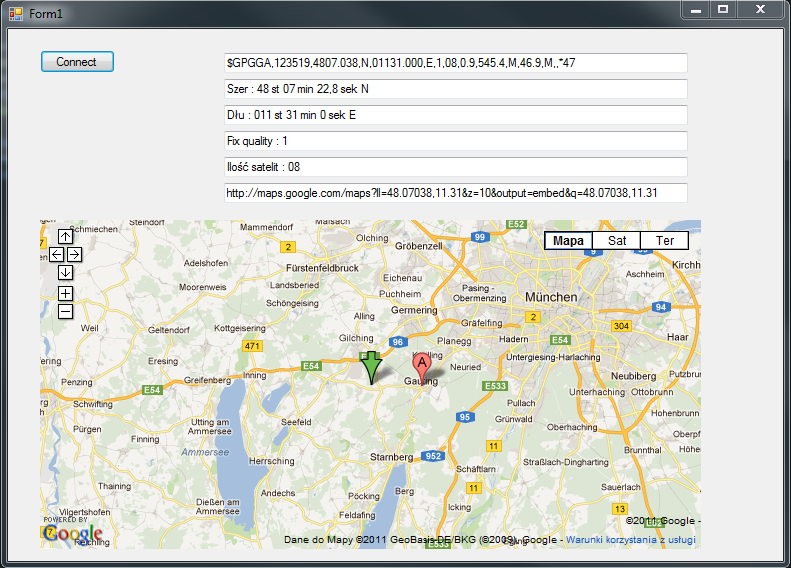
\includegraphics[width=\textwidth]{screen.PNG}
	\label{fig5}
      \end{center}
    \end{figure}

\end{document}